\RequirePackage{pdfmanagement}
\SetKeys[document/metadata]{pdfversion=1.7, pdfstandard=A-2u, lang=en-GB}
\input{preamble/pdfA-compliance/glyphtounicode}
\documentclass[11pt,a4paper]{report}

\newcommand*{\PaperTitle}{Every rational proportion of good vertices: \(\beta\)-Kirchhoff Šoltés graphs for all \(\beta<1\)}
\newcommand*{\PaperTitlePlain}{Every rational proportion of good vertices: beta-Kirchhoff Soltes graphs for all beta < 1}
\newcommand*{\PaperShortTitle}{\(\beta\)-Kirchhoff Šoltés graphs for all \(\beta<1\)}
\newcommand*{\PaperSubtitle}{chemistry-open-problems \textperiodcentered{} 31 October 2026 \textperiodcentered{} preliminary (verification pending)}
\newcommand*{\PaperCredits}{Solver: Claude Opus 5.5 (effort not recorded) \textperiodcentered{} Verification: pending}
\newcommand*{\PaperKeywords}{Kirchhoff index, resistance distance, Šoltés problem, good vertex, proportion of good vertices}
\input{chemop-preamble}
\addbibresource{references.bib}

\newcommand*{\Kf}{\operatorname{Kf}}
\newcommand*{\Rt}{\operatorname{Rt}}

\begin{document}
\makepapertitle

\begin{paperabstract}
A vertex \(v\) of a connected graph \(G\) is good if \(G-v\) is connected and \(\Kf(G-v)=\Kf(G)\), where \(\Kf\) is the
Kirchhoff index. Gottwald, Majstorović Ergotić and Došlić asked, for a fixed rational \(\beta\in(0,1]\), for an infinite
series of graphs in which at least a proportion \(\beta\) of the vertices are good; their best proportions tend to
\(2/3\). We prove that every rational \(\beta\in(0,1)\) is the exact proportion of good vertices of infinitely many
connected graphs. This settles their Problem~4 for every \(\beta<1\) and their Problem~5 for every \(\gamma\in(0,1]\), and
it answers their Problem~17: the exact values are the rationals in \((0,1]\) and the limiting values are all real numbers
in \((0,1]\). The graphs are a clique \(K_{ab+1}\) with one extra vertex (a hub) attached to each of \(a\) disjoint blocks
of \(b\) clique vertices, and a small rooted graph \(W\) glued at the clique vertex outside the blocks. The good vertices
are exactly the block vertices. Their goodness equation is linear in the transmission of \(W\), and all its denominators
are explicit products of small numbers, so it can be solved exactly. Explicit examples: a graph on 1772
vertices with proportion \(297/443>2/3\) and a graph on 2277 vertices with proportion exactly \(2/3\), both checked by exact
arithmetic on the actual Laplacian. The case \(\beta=1\) (the Kirchhoff Šoltés problem itself) is not addressed.
\end{paperabstract}

\section*{The question}

K. K. Gottwald, S. Majstorović Ergotić, T. Došlić, \emph{Šoltés problem for the Kirchhoff index of a graph}, Applied
Mathematics and Computation 510 (2026) 129694~\autocite{GMD2026} (arXiv:2609.13751). With
\(K(G)=\{v\in V(G):\Kf(G)=\Kf(G-v)\}\), they call \(G\) a \(\beta\)-Kirchhoff Šoltés graph if \(|K(G)|\ge\beta|V(G)|\), and
they ask (journal pp.~3 and~11):
\begin{openquote}
``Problem 4. For a fixed rational number \(\beta\in(0,1]\) construct an infinite series of \(\beta\)-Kirchhoff Šoltés graphs.''

``Problem 5. Given a fixed \(\gamma\in(0,1]\), construct an infinite series of graphs where the proportion of good vertices
increases and asymptotically approaches \(\gamma\) as the order of the graph grows.''

``Problem 17. Which (rational or irrational) numbers \(\gamma\in(0,1]\) appear either as exact or as limiting values of
proportions of good vertices with respect to the Kirchhoff Šoltés problem for simple undirected graphs?''
\end{openquote}
A vertex whose removal disconnects the graph is not good. The largest limiting proportion in~\autocite{GMD2026} is
\(2/3\), from splices of \(K_4-e\). The earlier stage of the present work~\autocite{ParentResult} proved that \(C_5\) is
the only connected graph with at most 10 vertices and proportion at least \(2/3\), and that splices of bounded branches
cannot exceed \(2/3\) (for branches with at most 9 vertices, by exact computation). It left \(\beta\ge2/3\) open.

\begin{theorem}\label{thm:main}
For every rational \(\beta\in(0,1)\) there are connected graphs \(G\) of arbitrarily large order with
\(|K(G)|=\beta\,|V(G)|\).
\end{theorem}

\begin{corollary}\label{cor:problems}
\begin{enumerate}
\item Problem~4 holds for every rational \(\beta\in(0,1)\).
\item Problem~5 holds for every real \(\gamma\in(0,1]\): there are graphs of strictly increasing orders whose proportions
of good vertices increase strictly and tend to \(\gamma\).
\item Problem~17: the exact proportions are exactly the rational numbers in \((0,1]\), and every real number in \((0,1]\) is
a limiting proportion.
\end{enumerate}
\end{corollary}
\begin{proof}
(1) follows from \zcref{thm:main}, since orders are unbounded. For (2) choose rationals \(\beta_1<\beta_2<\dots\) in
\((0,1)\) tending to \(\gamma\), and inductively a graph \(G_i\) with proportion exactly \(\beta_i\) and
\(|V(G_i)|>|V(G_{i-1})|\). (3) follows, with \(1\) attained by \(C_5\)~\autocite{GMD2026}; an exact proportion is
rational by definition.
\end{proof}

The case \(\beta=1\) of Problem~4 is the Kirchhoff Šoltés problem (Problem~3 of~\autocite{GMD2026}), which we do not
address~\autocite{SiblingKS}: all graphs below have cut vertices, so their proportion is below 1.

\section{Notation and the splice lemma}\label{sec:splice}

Graphs are finite, simple and connected. \(r_G(u,w)\) is the effective resistance between \(u\) and \(w\) when each edge is
a unit resistor, \(\Rt_G(u)=\sum_wr_G(u,w)\) is the transmission, and
\(\Kf(G)=\sum_{\{u,w\}}r_G(u,w)\)~\autocite{KleinRandic1993,GutmanMohar1996}. If \(L\) is the Laplacian of \(G\) and
\(L\varphi=e_s-e_t\), then \(r_G(s,t)=\varphi(s)-\varphi(t)\). We write \(\Delta_G(v)=\Kf(G)-\Kf(G-v)\) when \(G-v\) is
connected, so \(v\) is good iff \(\Delta_G(v)=0\).

A rooted graph \((Z,x)\) is a graph with a root \(x\). Put \(m_Z=|V(Z)|-1\) and \(T_Z=\Rt_Z(x)\). For \(z\ne x\) with \(Z-z\)
connected, let \(\delta_Z(z)=\Kf(Z)-\Kf(Z-z)\) and \(\rho_Z(z)=\Rt_{Z-z}(x)-\Rt_Z(x)\). The splice \(Z\oplus Z'\) identifies
the roots; \(m\) and \(T\) are additive under splicing.

\begin{lemma}[note={splice lemma}]\label{lem:splice}
(Lemma~1 of~\autocite{ParentResult}.) Let \(G=Z\oplus R\), and let \(z\ne x\) be a vertex of \(Z\). If \(Z-z\) is connected, then
\(\Delta_G(z)=\delta_Z(z)-m_R\,\rho_Z(z)+T_R\). If \(Z-z\) is disconnected, then \(z\) is a cut vertex of \(G\), so it is not
good.
\end{lemma}
\begin{proof}
Resistances inside \(Z\) and inside \(R\) are unchanged in \(G\), and \(r_G(u,w)=r_Z(u,x)+r_R(x,w)\) across \(x\). Hence
\(\Kf(Z\oplus R)=\Kf(Z)+\Kf(R)+m_RT_Z+m_ZT_R\). Subtract the same identity for \((Z-z)\oplus R\), in which
\(m_{Z-z}=m_Z-1\).
\end{proof}

\section{The clique with hubs}\label{sec:hubs}

Let \(U\) be a set of \(N\ge2\) vertices, split into blocks \(B_1,\dots,B_a\) of sizes \(b_i\ge1\) and a set \(C\) of hubless
vertices. The graph \(H\) is the clique on \(U\) together with hubs \(h_1,\dots,h_a\), where \(h_i\) is adjacent exactly to the
vertices of \(B_i\). Put \(x_i=1/b_i\), \(Y=\sum_ix_i\) and \(a'=a+|C|\). This class is closed under the deletion of a vertex
of \(U\), and under the deletion of a hub (the vertices of its block become hubless). It is what makes everything below
explicit: eliminating the hubs from the Laplacian leaves a matrix on \(U\) with the eigenvalues \(0\), \(N\) and \(N+1\) only,
whatever the block sizes.

\begin{lemma}\label{lem:res}
Let \(f\) be a function on \(V(H)\) with \(\sum f=0\), and let \(F_i=f(h_i)+\sum_{u\in B_i}f(u)\). Then \(L_H\varphi=f\) for
\[\varphi(h_i)=\frac{F_i}{b_iN}+\frac{f(h_i)}{b_i},\quad\varphi(u)=\frac{f(u)+\varphi(h_i)}{N+1}\ (u\in B_i),\quad
\varphi(c)=\frac{f(c)}N\ (c\in C).\]
Consequently, for \(u\in B_i\), \(u'\in B_j\), and hubless \(c\neq c'\):
\begin{align*}
r(u,u')&=\frac2{N+1}\ \ (i=j),&r(u,u')&=\frac{2+(x_i+x_j)/N}{N+1}\ \ (i\ne j),\\
r(h_i,u)&=x_i+\frac{1-x_i}{N+1},&r(h_i,u')&=x_i\frac{N+1}N+\frac{1+x_j/N}{N+1}\ \ (i\ne j),\\
r(h_i,h_j)&=(x_i+x_j)\frac{N+1}N\ \ (i\neq j),&r(c,c')&=\frac2N,\\
r(c,u)&=\frac1N+\frac{1+x_i/N}{N+1},&r(c,h_i)&=\frac1N+x_i\frac{N+1}N.
\end{align*}
\end{lemma}
\begin{proof}
From the definition, \(\sum_{u\in B_i}\varphi(u)=\bigl(F_i-f(h_i)+b_i\varphi(h_i)\bigr)/(N+1)=F_i/N\), so
\(\sum_U\varphi=\frac1N\bigl(\sum_iF_i+\sum_Cf\bigr)=0\). Hence \(L_H\varphi(u)=(N+1)\varphi(u)-\varphi(h_i)=f(u)\) on \(B_i\),
\(L_H\varphi(c)=N\varphi(c)=f(c)\) on \(C\), and \(L_H\varphi(h_i)=b_i\varphi(h_i)-F_i/N=f(h_i)\). The resistances follow by
taking \(f=e_s-e_t\) and \(r(s,t)=\varphi(s)-\varphi(t)\).
\end{proof}

A hubless vertex behaves in these formulas like a block of size 1 without its hub: \(r(c,u)\) and \(r(c,c')\) are the second
formula of the list with \(x=1\), and \(r(c,h_i)\) is the fourth with \(x_j=1\).

\begin{lemma}\label{lem:kf}
\[\Kf(H)=Y\,\frac{(N+1)(N+a-1)}N+(N+a-2)+\frac{(1+a')(1-a)}{N+1}+\frac{a(a'-2)}N,\]
and for a hubless vertex \(c\),
\[\Rt_H(c)=2+Y+\frac{Y+a+a'-2}N-\frac{1+a'}{N+1}.\]
\end{lemma}
\begin{proof}
Call parts the blocks and the singletons of \(C\), with \(x_P=1/|P|\). We use \(\sum_{P<P'}|P||P'|(x_P+x_{P'})=(a'-1)N\) and
sum the resistances of \zcref{lem:res}. Pairs in \(U\) give \(\bigl(N(N-1)+a'-1\bigr)/(N+1)\). A hub \(h_i\) and \(U\) give
\(1+\frac{N-1}{N+1}+x_i(N+1)-\frac{N+1}N+\frac{a'-1}{N(N+1)}\). Pairs of hubs give \((a-1)Y(N+1)/N\). Adding and using
\(N(N-1)+a'-1+a(N-a')=(N+1)(N+a-2)+(1+a')(1-a)\) gives \(\Kf(H)\). For \(\Rt_H(c)\), the vertices of \(U\) give
\(\bigl(2(N-1)+(N+a'-2)/N\bigr)/(N+1)\) and the hubs give \(a/N+Y(N+1)/N\); partial fractions in \(N\) give the formula.
\end{proof}

From now on \(H=H_{a,b}\), for \(a\ge2\), \(b\ge2\): all \(a\) blocks have size \(b\), and \(C=\{w\}\). So \(N=ab+1\),
\(a'=a+1\), \(Y=a/b\), and \(|V(H)|=ab+a+1\). Put \(B=b(b-1)\). Removing a block vertex \(v\) gives the parameters \(N-1\),
\(a\), \(a+1\), \(Y+1/B\). Removing a hub \(h\) gives \(N\), \(a-1\), \(a+b\), \(Y-1/b\). Let
\[\delta=\Kf(H)-\Kf(H-v),\qquad\rho=\Rt_{H-v}(w)-\Rt_H(w),\]
\[\delta_h=\Kf(H)-\Kf(H-h),\qquad\rho_h=\Rt_{H-h}(w)-\Rt_H(w).\]

\begin{lemma}\label{lem:delta}
These numbers do not depend on the choice of \(v\) or \(h\), and
\begin{align*}
\delta&=-\frac{2a}{B}+\frac{b^4-b^3-2b+1}{b^3(b-1)}+\frac{2(b-1)(b+2)}{b^2(ab+2)}\\
&\quad-\frac{(b+1)(2b^2-2b-1)}{b^3(ab+1)}+\frac1{ab^2(b-1)},\\
\rho&=\frac1{B}+\frac{2(b-1)}{b(ab+2)}-\frac{b^2-3b-1}{b^2(ab+1)}-\frac{b^2-b-1}{ab^2(b-1)},\\
\delta_h&=\frac{(N+1)(N+2a-2)}{bN}+1+\frac{ab-2a-2b}{N+1}-\frac{(a-1)(b-2)}N,\\
\rho_h&=-\frac1b+\frac{b-2-1/b}N-\frac{b-1}{N+1}.
\end{align*}
Moreover \(\delta_h\ge a-2\), and \(\rho_h<0\) when \(N\ge b\).
\end{lemma}
\begin{proof}
Substitute the parameters in \zcref{lem:kf}. These are identities between rational functions of \(a\) and \(b\); they are
checked symbolically, and on actual graphs, by \texttt{check\_formulas.py} (claims F3, F4). The estimates: the first term of
\(\delta_h\) is at least \(N/b\ge a\), the third is at least \(-2\) and the last at least \(-1\). In \(\rho_h\),
\((b-2-1/b)/N-(b-1)/(N+1)=\bigl((b-2-1/b)-N(1+1/b)\bigr)/\bigl(N(N+1)\bigr)<0\) when \(N\ge b\).
\end{proof}

So for fixed \(b\) and \(a\to\infty\): \(\delta=-2a/B+O(1)\) and \(\rho=1/B+O(1/a)\). In particular \(\delta<0\): for large
\(a\), deleting a block vertex raises the Kirchhoff index, because the resistance from its hub to the whole graph rises. A
branch glued at \(w\) raises \(\Delta\) back, and the denominators of \(\delta\) and \(\rho\) are small. That is the whole
idea.

\begin{figure}[ht]
\centering
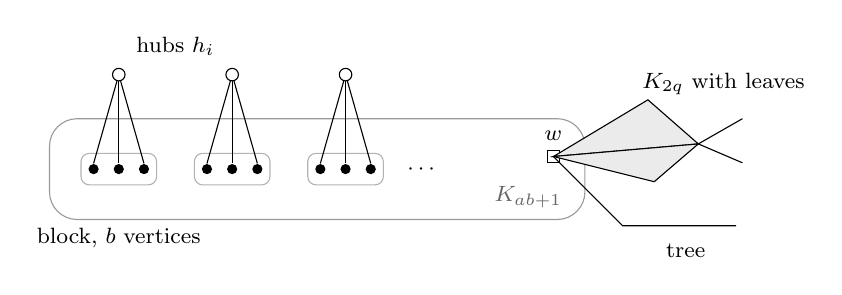
\begin{tikzpicture}[x=0.8cm,y=0.8cm,
  gd/.style={circle,fill=black,inner sep=1.3pt},
  hb/.style={circle,draw,fill=white,inner sep=1.6pt},
  rt/.style={rectangle,draw,fill=white,inner sep=2.2pt}]
\draw[black!40,rounded corners=10pt] (-0.6,-0.8) rectangle (7.9,0.8);
\node[font=\footnotesize,black!60] at (7.0,-0.45) {\(K_{ab+1}\)};
\foreach \k/\t in {0/0,1.8/1,3.6/2}{
  \draw[black!30,rounded corners=3pt] (\k-0.1,-0.25) rectangle (\k+1.1,0.25);
  \node[gd] (a\t) at (\k+0.1,0) {};
  \node[gd] (b\t) at (\k+0.5,0) {};
  \node[gd] (c\t) at (\k+0.9,0) {};
  \node[hb] (h\t) at (\k+0.5,1.5) {};
  \draw (h\t)--(a\t.north); \draw (h\t)--(b\t.north); \draw (h\t)--(c\t.north);
}
\node[font=\footnotesize] at (5.3,0) {\(\cdots\)};
\node[rt,label={[font=\footnotesize]above:\(w\)}] (w) at (7.4,0.2) {};
\node[font=\footnotesize] at (1.4,1.95) {hubs \(h_i\)};
\node[font=\footnotesize] at (0.5,-1.1) {block, \(b\) vertices};
\coordinate (p1) at (8.9,1.1); \coordinate (p2) at (9.7,0.4);\coordinate (p3) at (9.0,-0.2);
\draw[fill=black!8] (w.center)--(p1)--(p2)--cycle; \draw[fill=black!8] (w.center)--(p2)--(p3)--cycle;
\draw (p2)--(10.4,0.8); \draw (p2)--(10.4,0.1);
\node[font=\footnotesize] at (10.1,1.35) {\(K_{2q}\) with leaves};
\draw (w.center)--(8.5,-0.9)--(9.4,-0.9)--(10.3,-0.9);
\node[font=\footnotesize] at (9.5,-1.3) {tree};
\end{tikzpicture}
\caption{The graph \(G=H_{a,b}\oplus W\). The base is a clique on \(ab+1\) vertices. The black block vertices are the good
vertices. \(W\) is glued at the hubless vertex \(w\): cliques carrying the denominators, cliques that only add vertices, and
a tree that fixes the integer part of the transmission.}
\label{fig:construction}
\end{figure}

\section{Rooted graphs with prescribed order and transmission}\label{sec:rooted}

\begin{lemma}\label{lem:rooted}
\begin{enumerate}
\item\label{it:clique} For \(c\ge2\) let \(K_c\) be rooted at a vertex. Then \(m=c-1\), \(T=2(c-1)/c\), and for each non-root
vertex \(z\), \(\delta(z)=1\) and \(\rho(z)=-2/(c(c-1))\).
\item\label{it:gadget} For integers \(q\ge1\), \(j\ge0\), let \(Z(q,j)\) be \(K_{2q}\) rooted at \(x\), with \(j\) pendant
leaves attached to one fixed non-root vertex \(y\). Then \(m=2q-1+j\) and \(T=2-\frac1q+j\bigl(1+\frac1q\bigr)\). For a clique
vertex \(z\ne x,y\), with \(c=2q\),
\[\delta(z)=1+j+\frac{2j}{c(c-1)},\qquad\rho(z)=\frac{2(j-1)}{c(c-1)}.\]
\item\label{it:tree} For integers \(l\ge1\), \(l\le t\le l(l+1)/2\), there is a rooted tree with \(l\) non-root vertices and
\(T=t\).
\item\label{it:leaf} If \(z\) is a pendant vertex of \(Z\), \(z\ne x\), then \(\delta_Z(z)=\Rt_Z(z)>0\) and
\(\rho_Z(z)=-r_Z(x,z)<0\).
\end{enumerate}
\end{lemma}
\begin{proof}
(1) \(r=2/c\) in \(K_c\) and \(\Kf(K_c)=c-1\). (2) By \zcref{lem:splice}'s formula for \(\Kf\) of a splice at \(y\),
\(\Kf(Z(q,j))=(c-1)+j^2+2j(c-1)/c+j(c-1)\); replace \(c\) by \(c-1\) for \(Z-z\). Also
\(T=(c-1)2/c+j(1+2/c)\). (3) In a tree, \(T\) is the sum of the depths. Let \(k\) be the largest integer with \(k\le l\) and
\(k(k+1)/2+l-k\le t\). Take a path of \(k\) vertices from the root, and \(l-k\) further children of the root. If
\(e=t-k(k+1)/2-(l-k)\) is positive, then \(k<l\) and \(e<k\) by maximality of \(k\), and we move one of those children under the path
vertex at depth \(e\). (4) is immediate.
\end{proof}

\begin{lemma}\label{lem:moduli}
Let \(x\ge4\) be a multiple of \(b(b-1)\), let \(a=(x/b)(x^2-3x+1)\), and let
\[Q_0=b^2(b-1)\,x(x-2),\quad Q_1=x^2-3x+1,\]
\[Q_2=x^2-2x-1,\quad Q_3=x^2-x-1,\quad Q_4=x-1.\]
Then \(ab=xQ_1\), \(ab+1=Q_4Q_2\), \(ab+2=(x-2)Q_3\). The numbers \(Q_0,\dots,Q_4\) are pairwise coprime, and the denominators of
\(\delta\) and \(\rho\) divide \(D=Q_0Q_1Q_2Q_3Q_4\).
\end{lemma}
\begin{proof}
The three identities are expanded directly. Now \(x\) is even, since \(b(b-1)\) is, so \(Q_1,\dots,Q_4\) are odd, and each prime
factor of \(Q_0\) divides \(x(x-2)\). Modulo \(x\) the numbers \(Q_1,\dots,Q_4\) are \(1,-1,-1,-1\), and modulo \(x-2\) they
are \(-1,-1,1,1\); so each is coprime to \(Q_0\). Next \(Q_2-Q_1=x-2\), \(Q_3-Q_2=x\), and \(Q_3-Q_1=2(x-1)\); with the odd
numbers and the residues above, and \(Q_1\equiv Q_3\equiv-1\pmod{x-1}\), this gives \(\gcd(Q_1,Q_2)=\gcd(Q_2,Q_3)=\gcd(Q_1,Q_3)=1\)
and \(\gcd(Q_1,Q_4)=\gcd(Q_3,Q_4)=1\). Finally \(Q_2=(x-1)^2-2\) and \(Q_4\) is odd, so \(\gcd(Q_2,Q_4)=1\).

The denominators in \zcref{lem:delta} are \(b(b-1)\), \(b^3(b-1)\), \(b^2(ab+2)=b^2(x-2)Q_3\), \(b^3(ab+1)=b^3Q_4Q_2\),
\(ab^2(b-1)=b(b-1)xQ_1\), \(b(ab+2)\) and \(b^2(ab+1)\). Since \(b\mid x\), each of them divides \(D\).
\end{proof}

\section{Proof of \zcref{thm:main}}\label{sec:proof}

Let \(\beta=p/r\) in lowest terms, \(0<p<r\). Fix an integer \(b\ge2\) with \(b(r-p)>p\), and put \(B=b(b-1)\) and
\(\kappa=b(r-p)/p-1>0\). Let \(s\) run through the multiples of \(p\), and put \(x=Bs\), \(a=(b-1)s\,Q_1\) as in
\zcref{lem:moduli}, so \(p\mid a\). All implied constants below depend only on \(b\) and \(\beta\), and we let \(s\to\infty\).
Put
\[n=\frac{ab\,r}p\in\mathbb Z,\qquad m=n-(ab+a+1)=\kappa a-1.\]
We shall build a rooted graph \((W,w)\) with \(m_W=m\) and \(T_W=\tau:=m\rho-\delta\). Then \(G=H_{a,b}\oplus W\) has \(n\) vertices
and, by \zcref{lem:splice} with \(Z=H_{a,b}\), \(\Delta_G(v)=\delta-m\rho+\tau=0\) for each of the \(ab\) block vertices \(v\).

\emph{Sizes.} We have \(a\asymp x^3\). Let \(E=-\delta\), \(\Sigma=\sum_iQ_i=O(x^2)\) and
\(L=\lceil2\sqrt{E+1}\,\rceil=O(x^{3/2})\). By \zcref{lem:delta}, \(E=2a/B+O(1)\), so \(E\asymp x^3\), and \(m(\rho-1/B)=O(1)\). For
\(s\) large, let \(k\ge0\) be the largest integer with
\[m_r:=m-kB(2B-1)\ \ge\ 3\Sigma+L,\qquad\text{so}\qquad m_r<3\Sigma+L+2B^2.\]

\emph{Filler.} Let \(F\) be the splice of \(kB\) copies of \(K_{2B}\). By \zcref{lem:rooted}(\ref{it:clique}),
\(m_F=kB(2B-1)\) and \(T_F=k(2B-1)\in\mathbb Z\). Put
\[\tau'=\tau-T_F=E+m\Bigl(\rho-\frac1B\Bigr)+\frac{m_r}B.\]

\emph{Denominators.} By \zcref{lem:moduli}, \(D\tau'\in\mathbb Z\) and the \(Q_i\) are pairwise coprime, so there are integers
\(c_i\) with \(\tau'-\sum_ic_i/Q_i\in\mathbb Z\). Let \(0\le j_i<Q_i\) with \(j_i\equiv c_i+1\pmod{Q_i}\), and let
\(Z_i=Z(Q_i,j_i)\). By \zcref{lem:rooted}(\ref{it:gadget}), \(T_{Z_i}\equiv(j_i-1)/Q_i\equiv c_i/Q_i\pmod1\),
\(T_{Z_i}\le Q_i+2\le3Q_i\) and \(m_{Z_i}\le3Q_i\). Put \(m_g=\sum m_{Z_i}\le3\Sigma\) and \(T_g=\sum T_{Z_i}\le3\Sigma\).

\emph{Integer part.} Let \(l=m_r-m_g\ge L\) and \(t=\tau'-T_g\in\mathbb Z\). Since \(E\asymp x^3\) while
\(\Sigma,L,m(\rho-1/B)\) are \(O(x^2)\), for \(s\) large we get
\(l\le3\Sigma+L+2B^2\le E-O(1)-3\Sigma\le t\) and \(t\le E+O(1)+m_r/B\le2E+2\le L^2/2\le l(l+1)/2\). By
\zcref{lem:rooted}(\ref{it:tree}) there is a rooted tree \(\Theta\) with \(l\) non-root vertices and \(T_\Theta=t\).

\emph{Conclusion of the construction.} Let \(W=F\oplus Z_0\oplus\dots\oplus Z_4\oplus\Theta\), rooted at \(w\). Then
\(m_W=m_F+m_g+l=m\) and \(T_W=T_F+T_g+t=\tau\). So \(G\) has \(n\) vertices, and all \(ab\) block vertices are good. This
already proves Problem~4 for \(\beta\). It remains to show that \(G\) has no other good vertex.

\emph{No other good vertex.} The vertex \(w\) is a cut vertex, since \(m\ge1\). For a hub \(h\), \zcref{lem:splice} and
\zcref{lem:delta} give \(\Delta_G(h)=\delta_h-m\rho_h+T_W>0\). Let \(z\) be a vertex of \(W\) that is not a cut vertex of \(G\). It
lies in a branch \(Z\) of \(W\), one of the copies of \(K_{2B}\), one of the \(Z_i\), or \(\Theta\). Let \(R\) be the rest of \(G\), so
\(G=Z\oplus R\) and \(T_R\ge\Rt_H(w)\ge a/b\) by \zcref{lem:kf}. By \zcref{lem:splice},
\(\Delta_G(z)=\delta_Z(z)-m_R\rho_Z(z)+T_R\). If \(z\) is pendant, or \(Z\) is a clique (\(j_i=0\) included), then \(\delta_Z(z)>0\) and
\(\rho_Z(z)<0\) by \zcref{lem:rooted}, so \(\Delta_G(z)>0\). Non-pendant vertices of \(\Theta\) and the vertex \(y\) of \(Z_i\) for
\(j_i\ge1\) are cut vertices. The remaining case is a clique vertex \(z\ne y\) of \(Z_i\), with \(j_i\ge1\); then
\(\delta_{Z_i}(z)>0\) and, with \(c=2Q_i\), \(j_i\le Q_i-1\),
\[\rho_{Z_i}(z)=\frac{2(j_i-1)}{c(c-1)}\le\frac1{2Q_i},\qquad\text{so}\qquad
\Delta_G(z)\ge\frac ab-\frac n{2Q_i}=\frac ab\Bigl(1-\frac{b^2r}{2pQ_i}\Bigr)>0,\]
because \(Q_i\ge x-1\to\infty\). Hence \(K(G)\) is exactly the set of block vertices, \(|K(G)|=ab=\beta n\), and \(n\to\infty\)
with \(s\). \qed

\begin{remark}
\begin{enumerate}
\item Without the filler \(F\) one takes \(m=O(x^2)\) and gets proportions tending to \(b/(b+1)\) from below, which already
gives Problem~4. The filler only lowers the proportion to the exact value \(\beta\). Its vertices are nearly neutral, because
\(\rho\approx1/B\) and each vertex of \(K_{2B}\) has resistance \(1/B\) to \(w\).
\item The choice of \(x\) only serves to split the denominators \(a\), \(ab+1\), \(ab+2\) of \zcref{lem:delta} into factors of
size \(O(x^2)=o(E)\).
\item The barrier of~\autocite{ParentResult} concerns good vertices lying in a fixed finite family of branches at a cut vertex. Here
all good vertices lie in one branch at \(w\), and that branch has unbounded order, so there is no conflict.
\item The rook graph \(K_a\square K_b\) with hubs on the rows, studied in~\autocite{ParentResult}, has the same real behaviour.
There, though, the vertex-deleted graph has large irreducible denominators such as \(a^2b+ab^2-b-1\). The clique base
removes them: the class of \zcref{sec:hubs} is closed under deletion, and its Kirchhoff index depends only on \((N,a,a',Y)\).
\end{enumerate}
\end{remark}

\section{Explicit graphs}\label{sec:examples}

The proof above is not optimised. For \(\beta=2/3\), \(b=3\) it gives \(n=8.4\cdot10^7\). Smaller graphs come from the same
equation \(T_W=m\rho-\delta\) by factoring the denominators into prime powers (with cliques \(K_q\) for odd \(q\), where
\(r=2/q\)). \zcref{tab:examples} lists four of them. A gadget \((c,j)\) is \(K_c\) with \(j\) leaves on one vertex, and the
tree is the tree of \zcref{lem:rooted}(\ref{it:tree}).

\begin{table}[ht]
\centering\footnotesize
\begin{tabular}{llp{5.4cm}lll}
 & \(a,b\) & gadgets \((c,j)\) at \(w\) & tree \((l,t)\) & \(n\) & proportion\\ \hline
E1 & 396, 3 & (5,2) (7,6) (11,7) (17,8) (29,18) (41,10) & (32,94) & 1772 & \(297/443\approx0.6704\)\\
E2 & 506, 3 & (4,0) (9,2) (5,3) (49,3) (11,9) (19,10) (23,6) (31,23) & (53,133) & 2277 & \(2/3\)\\
E3 & 1116, 4 & (64,30) (27,6) (5,3) (7,6) (11,3) (19,12) (29,4) (31,12) (47,2) & (62,114) & 5952 & \(3/4\)\\
E4 & 705, 4 & (4,0) (9,0) (7,2) (13,9) (17,3) (31,25) (47,34) & (15,43) & 3735 & \(188/249\approx0.7550\)
\end{tabular}
\caption{Explicit graphs \(H_{a,b}\oplus W\). In each of them \(K(G)\) is exactly the set of block vertices.}
\label{tab:examples}
\end{table}

To our knowledge E1, E3 and E4 are the first connected graphs other than \(C_5\) with more than two thirds of their vertices
good. We make no claim of minimality: nothing has been searched systematically above \(n=10\). In exploration, a variant with \(W\)
glued at a hub gave \(n=1543\) and proportion \(1032/1543\); that graph is not part of the certificates.

\section{Limitations}\label{sec:limits}

\begin{itemize}
\item Problem~3 (\(\beta=1\)) is not addressed.
\item In \zcref{thm:main}, ``\(s\) large'' is not made explicit. This does not affect the theorem. \texttt{check\_construction.py}
carries out the construction with exact arithmetic for 13 values of \(\beta\) from \(1/100\) to \(99/100\), and confirms every
step on the actual numbers.
\item We did not determine the smallest graph with proportion above \(2/3\).
\item The graphs are very dense and have a cut vertex. We do not know a 2-connected family with proportion above \(2/3\).
\item The result has not yet been checked by an independent verifier.
\end{itemize}

\section{Computer verification}\label{sec:verif}

All claims are checked with exact rational arithmetic (Python fractions, python-flint) under Fedora 44 in WSL, with Python 3.12,
python-flint 0.6, sympy 1.14 and networkx 3. No floating-point value enters a claim. The scripts are in \texttt{scripts/} and the logs in
\texttt{certificates/}.
\begin{center}
\footnotesize
\begin{tabular}{p{3.7cm}p{7.9cm}l}
script & claims (PASS/FAIL, exit code) & time\\ \hline
\texttt{check\_formulas.py} & \zcref{lem:res,lem:kf,lem:delta,lem:splice,lem:rooted,lem:moduli}: symbolic identities, and
brute force on random graphs of the class & 1 min\\
\texttt{check\_construction.py} & the proof of \zcref{thm:main} on 78 parameter sets, 13 values of \(\beta\): counts, the
equation \(\Delta_G(v)=0\), all inequalities of the last step & 1 min\\
\texttt{check\_examples.py} & complete \(K(G)\) of E1--E4, every vertex type, through \zcref{lem:splice} & 1 min\\
\texttt{check\_direct.py small} & \(K(G)\) computed vertex by vertex on the actual Laplacian for 8 graphs with \(n\) from 24 to 400 & 3 min\\
\texttt{check\_direct.py family} & a graph produced by the proof itself (\(\beta=1/100\), \(b=2\), \(s=2\), \(n=2000\)), one vertex per class & 5 min\\
\texttt{check\_direct.py} with \texttt{E1}, \texttt{E2}, \texttt{E4}, \texttt{E3quick} & E1, E2, E4: exact inverse of the actual grounded Laplacian, one vertex per class;
E3: block vertex, hub and root & 8--90 min
\end{tabular}
\end{center}
\texttt{check\_direct.py} uses none of the closed forms of this paper: it builds the adjacency lists and inverts the grounded
Laplacian exactly. This is fast because the denominators of these graphs are small; the Kirchhoff index of E2 is
\(1134673709326253/1314329940\).

\paperreferences
\end{document}
